Sobre um sistema cartesiano considera-se uma malha formada por circunfer�ncias de raios com medidas dadas por n�meros naturais e por 12 semirretas com extremidades na origem, separadas por �ngulos de n rad, conforme a figura.

\begin{figure}[h]
\centering
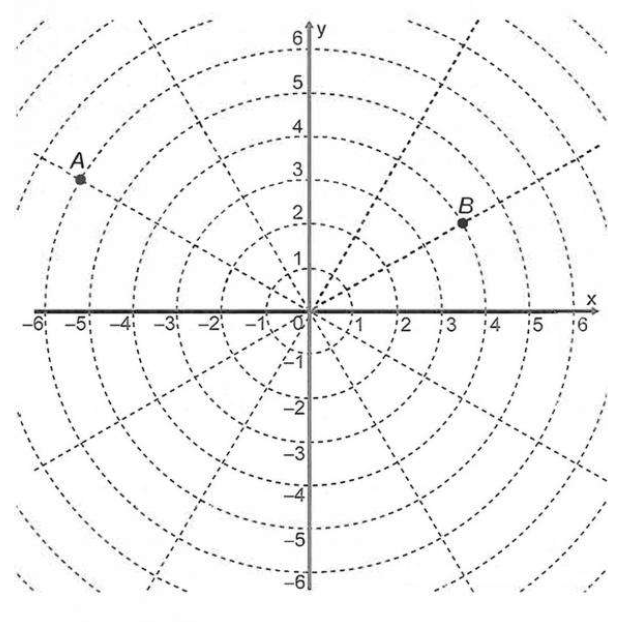
\includegraphics[width=8cm]{../figuras/q149-2018}
\end{figure}

Suponha que os objetos se desloquem apenas pelas semirretas e pelas circunfer�ncias dessa malha, n�o podendo passar pela origem (O ; O). 
Considere o valor de n com aproxima��o de, pelo menos, uma casa decimal. 
Para realizar o percurso mais curto poss�vel ao longo da malha, do ponto B at� o ponto A, um objeto deve percorrer uma dist�ncia igual a 

\begin{enumerate}
\item[a)]$\frac{2.\pi.1}{3}$
\item[b)]$\frac{2.\pi.2}{3}+6$
\item[c)]$\frac{2.\pi.3}{3}+4$
\item[d)]$\frac{2.\pi.4}{3}+2$
\item[e)]$\frac{2.\pi.5}{3}+2$
\end{enumerate}